\section{Privacy \& Datenschutz}

\subsection{Weshalb Privacy und Datenschutz}
Privatsphäre ist ein Menschenrecht. Alle modernen Demokratien schützen
diese! Im Grundsatz..

Um einen liberalen Lebensstil zu wahren, muss jeder Bürger selbst
entscheiden können \textbf{welche} Informationen er zur Verfügung stellt
und \textbf{wie} diese benutzt werden dürfen.


\subsection{Sphärentheorie}
Jeder entscheidet selbst, welche Daten/Information in welcher Sphäre
ist, weil jeder steht dazu was er macht.

\begin{figure}[H]
\centering
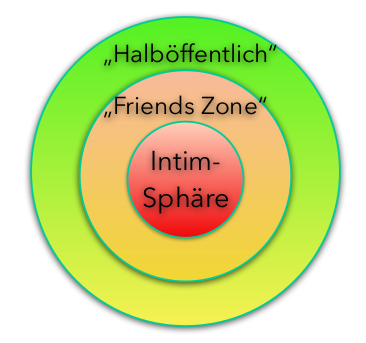
\includegraphics[width=.5\textwidth]{figures/sphaerentheorie.png}
\caption{Sphärentheorie}
\end{figure}

\textbf{Persönlichkeitsverletzung}:
\index{Persönlichkeitsverletzung}
Wenn Daten/Informationen von einer
Drittperson weitergegeben werden und somit ein Sphärenübertritt
stattfindet, spricht man von einer Persönlichkeitsverletzung.


\subsection{Schutz der Persönlichkeit}
\label{sec:Datenschutz-SchutzPersönlichkeit}

Ist im Art. 28 ZGB geregelt:\\
Wer in seiner Persönlichkeit \textbf{widerrechtlich} verletzt wird, kann zu
seinem Schutz gegen jeden, der in der Verletzung mitwirkt, das \textbf{Gericht}
anrufen.

\mbox{}\\
Eine Verletzung ist \textbf{widerrechtlich}, wenn sie nicht durch
\textbf{Einwilligung des Verletzten}, durch ein \textbf{überwiegend privates
oder öffentliches Interessen} oder durch \textbf{Gesetz} gerechtfertigt ist.


Dieses Gesetz stammt nicht vom Datenschutzgesetz, sondern vom
Zivilgesetzbuch.

Öffentliches Intresse besagt nicht, was die Öffentlichkeit
\textbf{interessiert} sondern was für die Öffentlichkeit
\textbf{relevant} ist.


\subsection{Datenschutz}
Als Datenschutz versteht man der Schutz der \textbf{Integrität} einer
Person vor Verletzungen Dritte.

Datenschutz ist\ldots{}

\begin{itemize}
	\tightlist
	\item Schutz der \textbf{informationellen Sebstbestimmung}
	\item Schutz der Persönlichkeit bei der Datenverarbeitung
	\item Schutz der Privatsphäre
	\item Schutz vor missbräuchlicher Datenverbreitung
\end{itemize}


\subsection{Gesetzliche Grundlagen}

\begin{itemize}
	\tightlist
	\item Schweizerische Bundesverfassung (Art. 13 BV)
	\item Bundesgesetz über den Datenschutz (DSG) und Verordnung dazu (VDSG)
	\item Zahlreiche datenschutzrechtliche Bestimmungen in anderen Gesetzen
	\item Kantonales und Gemeinderecht: zahlreiche Gesetze und Verordnungen
	\item International: Europäische Datenschutzrichtlinie bzw. -Grundverordnung
	(DSGVO/GDPR)
\end{itemize}

\subsection{Das schweizerische Datenschutzgesetz (DSG)}

\subsubsection{Geltungsbereich (Art. 2 DSG)}
\label{sec:Datenschutz-Geltungsbereich}

\begin{enumerate}
	\tightlist
	\item Dieses Gesetz gilt für das Bearbeiten von Daten \textbf{natürlicher
	und juristischer Personen} durch
	\begin{itemize}
		\tightlist
		\item private Personen;
		\item Bundesorgane.
	\end{itemize}
	\item Es ist nicht anwendbar auf:
	\begin{itemize}
		\tightlist
		\item Personendaten, die eine \textbf{natürliche Person ausschliesslich
		zum persönlichen Gebrauch bearbeitet und nicht an Aussenstehende bekannt
		gibt};
		\item Beratungen in den Eidgenössischen Räten und in den
		parlamentarischen Kommissionen;
		\item \textbf{hängige Zivilprozesse, Strafverfahren}, Verfahren der
		internationalen Rechtshilfe sowie staats- und verwaltungsrechtliche
		Verfahren mit Ausnahme erstinstanzlicher Verwaltungsverfahren;
		\item öffentliche Register des Privatrechtsverkehrs;
		\item Personendaten, die das Internationale Komitee vom Roten Kreuz
		bearbeitet.
	\end{itemize}
\end{enumerate}


\subsubsection{Begriffe \& Definitionen (Art. 3 DSG)}
\label{sec:Datenschutz-Begriffe}

\begin{description}
	\tightlist
	\item[Personendaten (Daten)] alle Angaben, die sich auf eine bestimmte oder
	bestimmbare Person beziehen.
	\item[betroffene Personen]  natürliche oder juristische Personen, über die
	Daten bearbeitet werden.
	\item[besonders schützenswerte Personendaten] Daten über:
	\begin{enumerate}
		\tightlist
		\item die religiösen, weltanschaulichen, politischen oder
		gewerkschaftlichen Ansichten oder Tätigkeiten
		\item die Gesundheit, die Intimsphäre oder die Rassenzugehörigkeit
		\item Massnahmen der sozialen Hilfe
		\item administrative oder strafrechtliche Verfolgungen und Sanktionen
	\end{enumerate}
	\item[Persönlichkeitsprofil] Eine Zusammenstellung von Daten, die eine
	Beurteilung wesentlicher Aspekte der Persönlichkeit einer natürlichen Person
	erlaubt.
	\item[Bearbeiten] Jeder Umgang mit Personendaten, unabhängig von den
	angewandten Mitteln und Verfahren, insbesondere das Beschaffen,
	Aufbewahren, Verwenden, Umarbeiten, Bekanntgeben, Archivieren oder
	Vernichten von Daten.
	\item[Bekanntgeben] Das Zugänglichmachen von Personendaten wie das
	Einsichtgewähren, Weitergeben oder Veröffentlichen.
	\item[Datensammlung] Jeder Bestand von Personendaten, der so
	aufgebaut ist, dass die Daten nach betroffenen Personen erschliessbar
	sind.
	\item[Bundesorgane]  Behörden und Dienststellen des Bundes sowie
	Personen, soweit sie mit öffentlichen Aufgaben des Bundes betraut sind.
	\item[Inhaber der Datensammlung] Private Personen oder Bundesorgane,
	die über den Zweck und den Inhalt der Datensammlung entscheiden.
\end{description}


\subsubsection{Datenschutzgrundsätze (Art. 4 DSG)}
\label{sec:Datenschutz-Datenschutzgrundsätze}

\begin{enumerate}
	\tightlist
	\item Personendaten dürfen nur \textbf{rechtmässig} bearbeitet werden.
	\item Ihre Bearbeitung hat nach Treu und Glauben zu erfolgen und muss
	\textbf{verhältnismässig} sein.
	\item Personendaten dürfen \textbf{nur zu dem Zweck bearbeitet werden, der
	bei der Beschaffung angegeben wurde, aus den Umständen ersichtlich
	oder gesetzlich vorgesehen ist.}
	\item Die Beschaffung von Personendaten und insbesondere der Zweck ihrer
	Bearbeitung müssen für die betroffene Person \textbf{erkennbar} sein.
	\item Ist für die Bearbeitung von Personendaten die Einwilligung der
	betroffenen Person erforderlich, so ist diese Einwilligung erst
	gültig, wenn sie \textbf{nach angemessener Information freiwillig
	erfolgt}. Bei der Bearbeitung von besonders schützenswerten
	Personendaten oder Persönlichkeitsprofilen muss die Einwilligung zudem
	\textbf{ausdrücklich} erfolgen.
\end{enumerate}


\subsubsection{Richtigkeit der Daten (Art. 5 DSG)}
\label{sec:Datenschutz-Richtigkeit}

\begin{enumerate}
	\tightlist
	\item Wer Personendaten bearbeitet, hat sich \textbf{über deren Richtigkeit
	zu vergewissern}. Er hat alle angemessenen Massnahmen zu treffen,
	damit die Daten \textbf{berichtigt oder vernichtet} werden, die im
	Hinblick auf den Zweck ihrer Beschaffung oder Bearbeitung unrichtig
	oder unvollständig sind.
	\item \textbf{Jede betroffene Person kann verlangen, dass unrichtige Daten
	berichtigt werden}.
\end{enumerate}

\subsubsection{Datensicherheit (Art. 7 DSG)}
\label{sec:Datenschutz-Datensicherheit}

\begin{enumerate}
	\tightlist
	\item Personendaten müssen durch \textbf{angemessene technische und
	organisatorische} Massnahmen gegen \textbf{unbefugtes Bearbeiten}
	geschützt werden.
	\item Der Bundesrat erlässt nähere Bestimmungen über die
	Mindestanforderungen an die Datensicherheit.
\end{enumerate}

\subsubsection{Grenzüberschreitende Bekanntgabe (Art. 6 DSG)}
\label{sec:Datenschutz-Grenzübergreifend}

\begin{enumerate}
	\tightlist
	\item Personendaten dürfen \textbf{nicht} ins \textbf{Ausland bekannt}
	gegeben werden, wenn dadurch die Persönlichkeit der betroffenen
	Personen \textbf{schwerwiegend gefährdet würde}, namentlich weil eine
	\textbf{Gesetzgebung} fehlt, die einen \textbf{angemessenen Schutz}
	gewährleistet.
	\item \ldots{} zahlreiche Voraussetzungen bei fehlen einer schützenden
	Gesetzgebung (z.B. nach Wegfall „Safe Harbor``)
\end{enumerate}

\subsubsection{Auskunftsrecht (Art. 8 DSG)}
\label{sec:Datenschutz-Auskunftsrecht}

\begin{enumerate}
	\tightlist
	\item Jede Person kann vom Inhaber einer Datensammlung \textbf{Auskunft}
	darüber verlangen, \textbf{ob Daten über sie bearbeitet} werden.
	\item Der Inhaber der Datensammlung \textbf{muss} der betroffenen Person
	\textbf{mitteilen}:
	\begin{itemize}
		\tightlist
		\item \textbf{alle} über sie in der Datensammlung \textbf{vorhandenen
		Daten} einschliesslich der verfügbaren Angaben über die
		\textbf{Herkunft} der Daten;
		\item den \textbf{Zweck} und gegebenenfalls die
		\textbf{Rechtsgrundlagen} des Bearbeitens sowie die Kategorien der
		bearbeiteten Personendaten, der an der Sammlung Beteiligten und der
		\textbf{Datenempfänger}.
	\end{itemize}
	\item Daten über die Gesundheit kann der Inhaber der Datensammlung der
	betroffenen Person durch einen von ihr bezeichneten Arzt mitteilen
	lassen.
	\item Lässt der Inhaber der Datensammlung Personendaten durch einen
	\textbf{Dritten bearbeiten}, so bleibt er \textbf{auskunftspflichtig}.
	Der Dritte ist auskunftspflichtig, wenn er den Inhaber nicht bekannt
	gibt oder dieser keinen Wohnsitz in der Schweiz hat.
	\item Die Auskunft ist in der Regel \textbf{schriftlich}, in Form eines
	Ausdrucks oder einer Fotokopie sowie \textbf{kostenlos} zu erteilen.
	Der Bundesrat regelt die Ausnahmen.
	\item \textbf{Niemand kann im Voraus auf das Auskunftsrecht verzichten.}
\end{enumerate}

\subsubsection{Informationspflicht beim Beschaffen von besonders
schützenswerten Personendaten und Persönlichkeitsprofilen (Art. 14 DSG)}
\label{sec:Datenschutz-Informationspflicht}

\begin{enumerate}
	\tightlist
	\item Der Inhaber der Datensammlung \textbf{ist verpflichtet}, die
	betroffene Person über die Beschaffung von besonders schützenswerten
	Personendaten oder Persönlichkeitsprofilen \textbf{zu informieren};
	diese Informationspflicht gilt auch dann, wenn die Daten bei Dritten
	beschafft werden.
	\item Der betroffenen Person sind mindestens mitzuteilen:
	\begin{itemize}
		\tightlist
		\item der \textbf{Inhaber der Datensammlung};
		\item der \textbf{Zweck} des Bearbeitens;
		\item die \textbf{Kategorien der Datenempfänger}, wenn eine
		Datenbekanntgabe vorgesehen ist.
	\end{itemize}
	\item Werden die Daten nicht bei der betroffenen Person beschafft, so hat
	deren Information \textbf{spätestens bei der Speicherung} der Daten
	oder, wenn die Daten nicht gespeichert werden, mit ihrer
	\textbf{ersten Bekanntgabe} an Dritte zu erfolgen.
	\item Die Informationspflicht des Inhabers der Datensammlung entfällt, wenn
	die betroffene Person bereits informiert wurde oder, in Fällen nach
	Absatz 3, wenn:
	\begin{itemize}
		\tightlist
		\item die Speicherung oder die Bekanntgabe der Daten ausdrücklich im
		Gesetz vorgesehen ist; oder
		\item die Information nicht oder nur mit unverhältnismässigem Aufwand
		möglich ist.
	\end{itemize}
	\item Der Inhaber der Datensammlung kann die Information unter den in
	Artikel 9 Absätze 1 und 4 genannten Voraussetzungen verweigern,	einschränken
	oder aufschieben
\end{enumerate}


\subsubsection{Verletzung der Auskunfts-, Melde- und Mitwirkungspflichten
(Art. 34 DSG)}
\label{sec:Datenschutz-Strafe}

\begin{enumerate}
	\tightlist
	\item Mit \textbf{Busse} werden \textbf{private Personen} auf Antrag
	bestraft:
	\begin{itemize}
		\tightlist
		\item die ihre Pflichten nach den Artikeln 8 - 10 und 14 verletzen, indem
		sie vorsätzlich eine falsche oder eine unvollständige Auskunft
		erteilen.
		\item die es \textbf{vorsätzlich} unterlassen:
		\begin{itemize}
			\tightlist
			\item die betroffene Person nach Artikel 14 Absatz 1 zu informieren,
			oder
			\item ihr die Angaben nach Artikel 14 Absatz 2 zu liefern.
		\end{itemize}
	\end{itemize}
	\item Mit Busse werden \textbf{private Personen} bestraft, die vorsätzlich:
	\begin{itemize}
		\tightlist
		\item die \textbf{Information} nach Artikel 6 Absatz 3 oder die
		\textbf{Meldung} nach Artikel 11a \textbf{unterlassen} oder dabei
		\textbf{vorsätzlich falsche Angaben machen};
		\item dem Beauftragten bei der Abklärung eines Sachverhaltes (Art. 29)
		\textbf{falsche Auskünfte} erteilen oder die \textbf{Mitwirkung}
		verweigern.
	\end{itemize}
\end{enumerate}

\subsubsection{Verletzung der beruflichen Schweigepflicht (Art. 35 DSG)}
\label{sec:Datenschutz-Schweigepflicht}

\begin{enumerate}
	\tightlist
	\item Wer \textbf{vorsätzlich geheime, besonders schützenswerte
	Personendaten oder Persönlichkeitsprofile} unbefugt bekannt gibt, von denen
	er bei der Ausübung seines Berufes, der die Kenntnis solcher Daten
	erfordert, erfahren hat, wird \textbf{auf Antrag mit Busse bestraft}.
	\item Gleich wird bestraft, wer \textbf{vorsätzlich} geheime, besonders
	schützenswerte Personendaten oder Persönlichkeitsprofile \textbf{unbefugt}
	bekannt gibt, von denen er \textbf{bei der Tätigkeit für den
	Geheimhaltungspflichtigen} oder während der \textbf{Ausbildung} bei diesem
	erfahren hat.
	\item Das unbefugte Bekanntgeben geheimer, besonders schützenswerter
	Personendaten oder	Persönlichkeitsprofile ist \textbf{auch nach Beendigung
	der Berufsausübung oder der	Ausbildung strafbar}.
\end{enumerate}

\subsubsection{Datenverarbeitung durch Dritte (Art. 10A DSG)}
\label{sec:Datenschutz-Dritte}

\begin{enumerate}
	\tightlist
	\item Das Bearbeiten von Personendaten kann \textbf{durch Vereinbarung oder
	Gesetz}	Dritten	übertragen werden, wenn:
	\begin{itemize}
		\tightlist
		\item die Daten nur so bearbeitet werden, \textbf{wie der Auftraggeber
		selbst es tun dürfte}; und
		\item \textbf{keine gesetzliche} oder \textbf{vertragliche
		Geheimhaltungspflicht} es verbietet.
	\end{itemize}
	\item Der Auftraggeber muss sich insbesondere \textbf{vergewissern}, dass
	der Dritte die \textbf{Datensicherheit} gewährleistet.
	\item Dritte können dieselben Rechtfertigungsgründe geltend machen wie der
	Auftraggeber.
\end{enumerate}

\subsection{Datenschutz im Arbeitsverhältnis (Art. 328B OR)}
\label{sec:Datenschutz-Arbetsverhältnis}
Der Arbeitgeber darf Daten über den Arbeitnehmer nur
bearbeiten, soweit sie dessen \textbf{Eignung} für das
Arbeitsverhältnis betreffen oder zur\textbf{ Durchführung des
Arbeitsvertrages erforderlich} sind. Im Übrigen gelten die
Bestimmungen des Bundesgesetzes vom 19. Juni 1992 über
den Datenschutz.
